\documentclass[a4paper]{article}

\title{PH2255 Course:\\
Introduction to Statistical Methods\\Exercise 4}
\author{Thomas Bass}
\date{22 January 2021}

% LaTeX preambule: loading relevant packages, configuring Python listings
\usepackage{graphicx}
\usepackage{amsmath}
\usepackage{color}
\usepackage{listings}
\usepackage{hyperref}
\usepackage{bm}
\usepackage{amssymb}

\definecolor{dkgreen}{rgb}{0,0.6,0}
\definecolor{gray}{rgb}{0.5,0.5,0.5}
\definecolor{mauve}{rgb}{0.58,0,0.82}

% Settings for colour-coding and formatting Python code:
\lstset{
  language=Python,                % the language of the code
  basicstyle=\footnotesize,           % the size of the fonts that are used for the code
  numbers=left,                   % where to put the line-numbers
  numberstyle=\tiny\color{gray},  % the style that is used for the line-numbers
  stepnumber=5,                   % the step between two line-numbers. If it's 1, each line
                                  % will be numbered
  numbersep=5pt,                  % how far the line-numbers are from the code
  backgroundcolor=\color{white},      % choose the background color. You must add \usepackage{color}
  showspaces=false,               % show spaces adding particular underscores
  showstringspaces=false,         % underline spaces within strings
  showtabs=false,                 % show tabs within strings adding particular underscores
  frame=single,                   % adds a frame around the code
  rulecolor=\color{black},        % if not set, the frame-color may be changed on line-breaks within not-black text (e.g. commens (green here))
  tabsize=2,                      % sets default tabsize to 2 spaces
  captionpos=b,                   % sets the caption-position to bottom
  breaklines=true,                % sets automatic line breaking
  breakatwhitespace=false,        % sets if automatic breaks should only happen at whitespace
  title=\lstname,                   % show the filename of files included with \lstinputlisting;
                                  % also try caption instead of title
  keywordstyle=\color{blue},          % keyword style
  commentstyle=\color{dkgreen},       % comment style
  stringstyle=\color{mauve},         % string literal style
  escapeinside={\%*}{*)},            % if you want to add LaTeX within your code
  morekeywords={*,...}               % if you want to add more keywords to the set
}

\begin{document}
\maketitle

\subsection{Question 1}
Using Kirchoff's first law to sum the voltages around the LCR circuit:
\begin{equation}
V = IZ = I\left(R+i\omega L+\frac{•}{•}\omega C}\right)
\end{equation}
We can rewrite this in differential form:
\begin{equation}
L\ddot{q}+r\dot{q}+\frac1Cq=0
\end{equation}
This is in the same form as a damped mechanical oscillator $\ddot{q}+\gamma\dot{q}+\omega_0^2q=0$
Therefore $\omega_0=\sqrt{1/LC}$
From definition $\omega=\frac{2\pi}T=2\pi f$
\begin{equation}
f_0=\frac1{2\pi}\sqrt{\frac1{LC}}
\end{equation}

\subsection{Question 2}
Using values of $L=5mH=5\times10^{-3}H$ and $C=1nF=1\times10^{-9}F$:

$f_0=71,176.25Hz$

\subsection{Question 3}
For $\Delta\phi=0$, $f=71.18kHz$

Peak-to-peak voltages:

CH1: $1.463 V$

CH2: $1.082 V$

$\therefore V_2/V_1=0.7395$

This small $$\sim10Hz$$ discrepancy comes from additional impedance from the connections/wires in the circuit.

\subsection{Question 4}

Starting frequency $f_\text{min}=60kHz$, at $V_2/V_1=0.1296$

Ending frequency $f_\text{max}=82kHz$, at $V_2/V_1=0.1357$

\subsection{Question 6}
\begin{equation}
|Z|=\sqrt{R^2+(\omega L-1/\omega C)^2}
\end{equation}

At resonance, $\omega L-1/\omega C=0$, therefore that term drops out of the equation, giving us a minimum value $|Z|=R$.

At high frequencies, the Inductor term $\omega L$ dominates.

At low frequencies, the Capacitor term $1/\omega C$ dominates.

\subsection{Question 7}
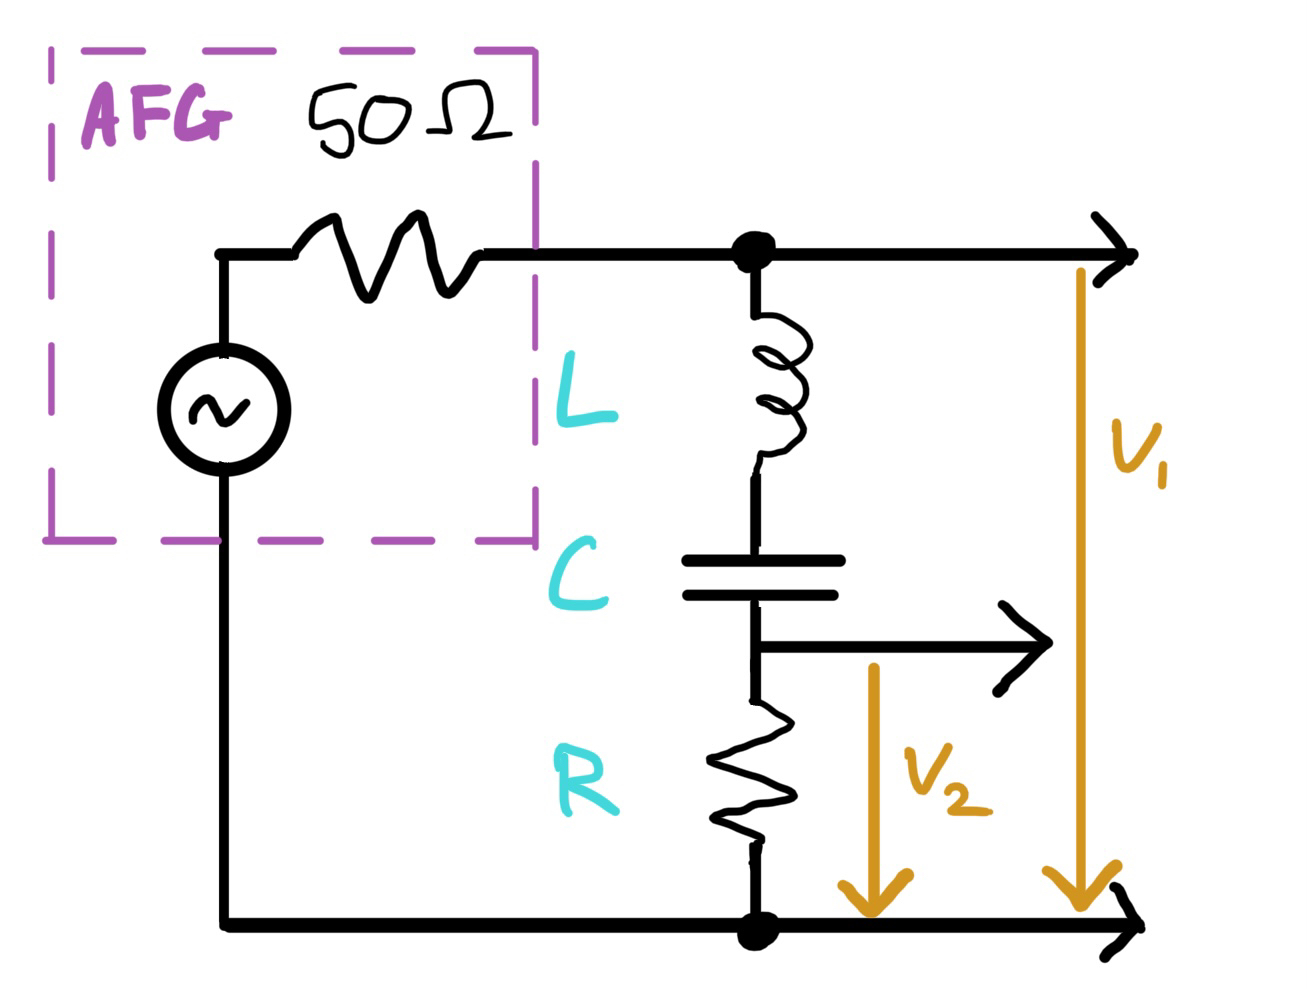
\includegraphics[scale=0.2]{circuit.png}

\subsection{Question 8}
\begin{figure}[h]
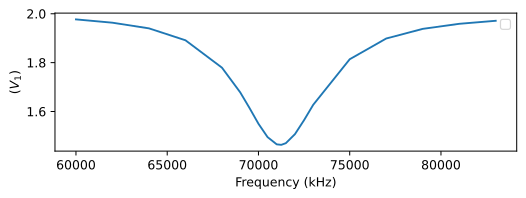
\includegraphics[scale=0.8]{v1.png}
\caption{The voltage $V_1$ plotted against the driving frequency of the AFG}
\end{figure}

This plot, showing how $V_1$ changes as we change the AFG frequency, takes the form of a $y=\sqrt x$ function. As $V_1$ takes the potential difference over the entire LCR circuit, we include both the resistance, inductance, and capacitance of the three components into account when using Equation 4.

We need to measure the $V_1$ across the whole circuit, rather than using the AFG's setting, as there are impedance/resistive effects from the wires connecting the components, and the electronics inside the AFG.

We can apply Ohm's law ($V=IR$) to the resistor, using $V_2$, to find the current through the resistor. As the circuit is in series, the current through the resistor is the same as the current through each component of the circuit.

\subsection{Question 9}
\begin{figure}[h]
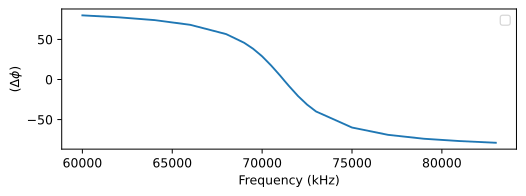
\includegraphics[scale=0.8]{phase.png}
\caption{The phase different $\Delta\phi$ plotted against the driving frequency of the AFG}
\end{figure}

From the equation given in the lab script:
\begin{equation}
\Delta\phi=\tan^{-1}[(\omega L-1/\omega C)/R]
\end{equation}
We can see that as $f\rightarrow0$, the arctan will approach 90 degrees, and as $f\rightarrow\infty$, the arctan approaches -90 degrees.

\subsection{Question 10}
\begin{figure}[h]
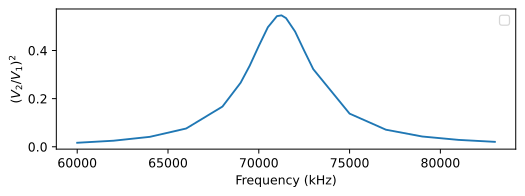
\includegraphics[scale=0.8]{qfac.png}
\caption{$(V_2/V_1)^2$ plotted against the driving frequency of the AFG}
\end{figure}

Estimating values either side of resonance where $(V_2/V_1)^2$ are at half maximum:

$f_1\approx69050 Hz$

$f_2\approx74500 Hz$

Using these, we can estimate the quality factor of the resonance using the equation provided in the lab script:
\begin{equation}
Q=\frac{\omega_0}{\Delta\omega}=\frac{f_0}{\Delta f}
\end{equation}
Where $\Delta f=f_2-f_1$

Using this, we obtain a value of $Q=13.06$

However, if we use the equation involving $L$ and $R$:
\begin{equation}
Q=\frac{\omega_1L}R
\end{equation}
We obtain a value of $Q=3.56$. While these differ, both are above the critical $Q=\frac12$ value, indicating that this is an underdamped system. 

\subsection{Question 11}
Using Equation 3 to find an estimate of $f_0$ for a system with $L=5 mH$, $C=1 nF$, and $R-200 \Omega$, we obtain $f_0=71,176.25 Hz$, the same value as before. This is because we are only changing the resistor, which has no effect using Equation 3. Using the AFG simulator, we do in fact obtain the same experimental value of $f_0$. Because of this, we can use the same $f_\text{max}$ and $f_\text{min}$ as before.
\begin{figure}[h]
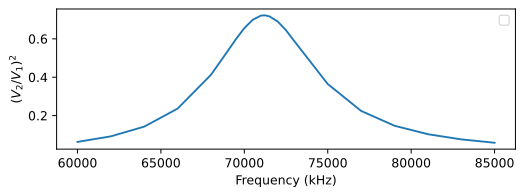
\includegraphics[scale=0.8]{qfac2.png}
\caption{$(V_2/V_1)^2$ plotted against the driving frequency of the AFG}
\end{figure}

If we again estimate $f_1$ and $f_2$ at half-maximum height:

$f_1=66500 Hz$

$f_2=75050 Hz$

From these values, we obtain a value of $Q=8.32$, again an underdamped system. If we use Equation 7, we obtain a value of $Q=1.78$
\newpage
\subsection{Question 12}
\begin{figure}[!h]
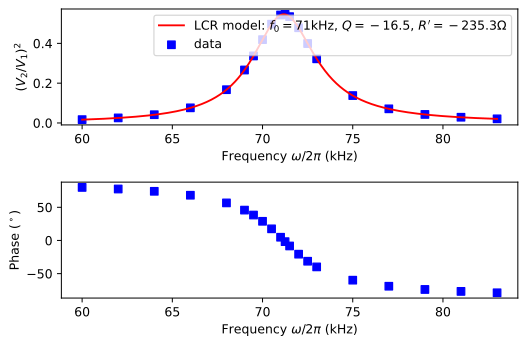
\includegraphics[scale=0.8]{res1.png}
\caption{$(V_2/V_1)^2$ plotted against the driving frequency of the AFG for $L=5\times10^{-3} H$, $C=1\times10^{-9}$, and  $R=100 \Omega$, and the fitted curve}
\end{figure}
\begin{figure}[!h]
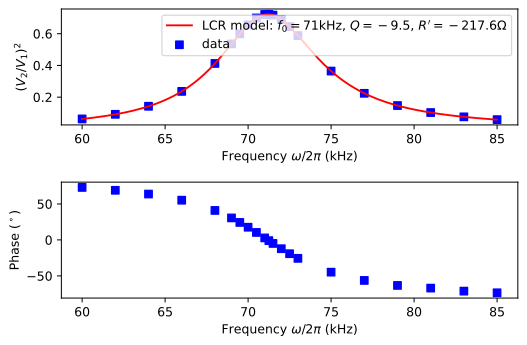
\includegraphics[scale=0.8]{res2.png}
\caption{$(V_2/V_1)^2$ plotted against the driving frequency of the AFG for $L=5\times10^{-3} H$, $C=1\times10^{-9}$, and  $R=200 \Omega$, and the fitted curve}
\end{figure}

\subsection{Question 13}

For the first fit, the values obtained were $f_0=71.18kHz$, $Q=-16.49$, and $R'=-235.27$. 

For the second fit, these values were $f_0=71.18kHz$, $Q=-9.48$, and $R'=-217.56$.

These values can be related to $R$, $L$, and $C$ using the following equations:
\begin{equation}
Q=\omega_0L/(R+R')
\end{equation}
\begin{equation}
\omega_0=\sqrt{\frac1{LC}}
\end{equation}

\end{document}
